\documentclass[a4paper,12pt]{article}   % Dokumentklass: artikel, A4, 12 pt
                                        % [a4paper,12pt] är valfria parametrar
                                        % och kan tas bort

% Det finns flera olika LaTeX-kompilatorer. Två vanliga är pdfLaTeX och XeLaTeX.
%  - pdfLaTeX är standard för de flesta dokument och är snabb och pålitlig,
%    men har begränsat Unicode-stöd.
%  - XeLaTeX erbjuder fullt Unicode-stöd och möjligheten att använda
%    systemtypsnitt, vilket gör det lämpligt för internationella dokument.


% Endast för pdfLaTeX. Behövs inte för XeLaTeX, eftersom den använder
% Unicode och systemets redan installerade typsnitt (fonts).
\usepackage[utf8]{inputenc}             % UTF-8 teckenkodning för pdfLaTeX
\usepackage[T1]{fontenc}                % Teckenuppsättning för pdfLaTeX

% Behövs för både för pdfLaTeX och XeLaTeX
\usepackage[swedish]{babel}             % Svensk språkstil och avstavning

% Om du vill använda särskillda typsnitt med XeLaTeX, använd följande:
% \usepackage{fontspec}                  % För att kunna använda typsnitt
% \setmainfont{Latin Modern Roman}       % Sätt huvudtypsnittet

% Övriga paket
\usepackage{graphicx}                   % Hantera bilder
\usepackage{tcolorbox}                  % Färgade ramar/lådor
% \usepackage{amsmath}                    % Mer avancerat matematikstöd,
%                                         % t.ex. flerradiga ekvationer,
%                                         % matriser, anpassade operatorer
%                                         % och bättre layout, men behövs
%                                         % inte för detta dokument

% För att inkludera källkod kan man använda 'verbatim',
% men 'listings' ger ofta bättre resultat
\usepackage{listings}                   % Källkodshantering

% Konfigurera hur kodlistningar ska visas
\lstset{
  language=Scala,                       % Använder Scala för syntaxmarkering
  basicstyle=\ttfamily\footnotesize,    % Använder monospace teckensnitt
                                        % (Consolas), samt mindre textstorlek
  keywordstyle=\color{blue}\bfseries,   % Färglägger nyckelord
  stringstyle=\color{orange},           % Färglägger strängar i orange
  commentstyle=\color{gray}\itshape,    % Färglägger kommentarer
  showstringspaces=false,               % Visar inte mellanslag i strängar
  numbers=left,                         % Visar radnummer till vänster
  numberstyle=\tiny\color{gray},        % Gör radnummer små och grå
  stepnumber=1,                         % Visar varje radnummer
  tabsize=2,                            % Antal mellanslag i en tabb
  breaklines=true,                      % Radbrytning vid behov
  frame=single,                         % Ram runt koden
  columns=fullflexible,                 % Flexibel bredd på bokstäverna 
  keepspaces=true,                      % Behåller mellanslag i koden
  fontadjust=true,                      % Autojusterar fontstorlek vid behov
}


\usepackage{enumitem} % Anpassade listor
% Anpassa hur 'description' listor ser ut
\setlist[description]{
    leftmargin=2.3cm,   % Vänstermarginal
    rightmargin=1cm,    % Högermarginal
    labelindent=1cm,    % Etikettindrag
    labelwidth=1cm,     % Etikettbredd
    align=right,        % Högerjustera etikett
    labelsep=3mm        % Avstånd mellan etikett och beskrivning
}


\title{Effektivitet i Scala: Sorteringsalgoritmer}
\author{Fiktiv Författare}
\date{12 september 2024}

\begin{document}

\maketitle              % Skriv ut titel, författare och datum

\begin{tcolorbox}[title=Notera]
    Denna artikel är primärt genererad med hjälp av AI-verktyg, och sedan manuellt kontrollerad och justerad. Alla data och mätningar är påhittade för övningsändamål.
\end{tcolorbox}

\section{Introduktion}

Scala är ett populärt språk som kombinerar funktionell och objektorienterad programmering. I denna artikel utvärderar vi effektiviteten hos olika sorteringsalgoritmer när de används i Scala. Speciellt fokuserar vi på sorteringsalgoritmerna \emph{QuickSort} och \emph{MergeSort}.

\section{O-notation}

Innan vi börjar prata om algoritmers tidseffektivitet behöver vi förstå så kallad \emph{O-notation}. O-notation (ibland kallad ``stora O-notation'' eller ``big O notation'' på engelska) är ett sätt att beskriva hur effektiv en algoritm är när det gäller exekveringstid, beroende på mängden data som algoritmen hanterar -- så kallad \emph{tidskomplexitet}. Den används ofta inom datavetenskap för att klassificera algoritmer baserat på deras prestanda, särskilt för stora inmatningsstorlekar.

O-notationen uttrycker hur algoritmens tid växer som en funktion av storleken på indata, vanligtvis betecknad som $n$. Till exempel, om en algoritm har en tidskomplexitet på $O(n)$, betyder det att tiden det tar att utföra algoritmen ökar linjärt med storleken på indata. O:et uttalas ofta som ``ordo'', alltså ``ordo n'' för $O(n)$ eller ``ordo n log n'' för $O(n \log n)$.

\subsection{Vanliga O-klasser}

Här är några av de vanligaste O-notationerna och vad de representerar:

\begin{description}
    \item[$O(1)$] Konstant tid -- Algoritmen tar samma tid oavsett storleken på indata.
    \item[$O(n)$] Linjär tid -- Tiden ökar direkt proportionellt mot storleken på indata. En dubbling av indata leder till en dubbling av exekveringstiden.
    \item[$O(\log n)$] Logaritmisk tid -- Tiden ökar mycket långsamt när indata växer. Vanligt i effektiva sökalgoritmer.
    \item[$O(n \log n)$] Linjär-logaritmisk tid -- Vanligt för många effektiva sorteringsalgoritmer, som exempelvis MergeSort.
    \item[$O(n^2)$] Kvadratisk tid -- Tiden växer kvadratiskt med indata; ofta sett i enklare sorteringsalgoritmer som Bubble Sort. En dubbling av indata leder till en fyrdubbling av exekveringstiden.
    \item[$O(2^n)$] Exponentiell tid -- Tiden växer mycket snabbt med storleken på indata; vanligt i vissa rekursiva algoritmer.
\end{description}

\subsection{Exempel}

Anta att vi har en sorteringsalgoritm som tar en lista med $n$ tal och jämför varje tal med varje annat tal för att avgöra ordningen. Denna algoritm skulle ha en tidskomplexitet på $O(n^2)$ eftersom varje element ($n$ stycken) jämförs med alla andra element ($n$ stycken)\footnote{Produkten blir egentligen $n\cdot(n-1)$, men konstanta värden ignoreras i O-notation eftersom de inte spelar någon roll när $n$ går mot ett stort värde.}.

O-notationen hjälper oss att förstå och förutsäga hur algoritmer beter sig när datamängden växer, och är därför ett ovärderligt verktyg vid val av algoritmer och datastrukturer.


\section{Sorteringsalgoritmer}

Sortering är en grundläggande operation inom datavetenskap, och olika algoritmer har olika prestanda beroende på data och sammanhang. Två av de vanligaste algoritmerna är \emph{QuickSort} och \emph{MergeSort}.

\subsection{Jämförelse av QuickSort och MergeSort}

QuickSort är en snabb sorteringsalgoritm som fungerar bra i genomsnittsfallet med tidskomplexiteten $O(n \log n)$. Den kan dock prestera dåligt i det värsta fallet, med en tidskomplexitet på $O(n^2)$, om pivotvalet är ogynnsamt. MergeSort, å andra sidan, har alltid en tidskomplexitet på $O(n \log n)$, vilket gör den stabilare men ibland långsammare på grund av dess behov av extra minnesutrymme.

I tabell~\ref{tab:sorteringsalgoritmer} nedan jämförs prestandan hos QuickSort och MergeSort för olika indata. Se Appendix~\ref{app:scala_impl} för implementationen i Scala. \emph{(Notera igen att datan är påhittad för övningsändamål.)}

\begin{table}[h]
    \centering
    \begin{tabular}{r|r|r|r|r}
        Algoritm  & Indatastorlek ($n$) & Indatatyp   & Tid ($\mu s$) & Minne (MB) \\
        \hline
        \hline
        QuickSort & 1000                & Slumpmässig & 12       & 5          \\
        QuickSort & 1000                & Sorterad    & 1        & 5          \\
        QuickSort & 1000                & Omvänd      & 30       & 5          \\
        \hline
        QuickSort & 10000               & Slumpmässig & 150      & 5          \\
        QuickSort & 10000               & Sorterad    & 2        & 5          \\
        QuickSort & 10000               & Omvänd      & 450      & 5          \\
        \hline
        QuickSort & 100000              & Slumpmässig & 1800     & 5          \\
        QuickSort & 100000              & Sorterad    & 10       & 5          \\
        QuickSort & 100000              & Omvänd      & 9000     & 5          \\
        \hline
        \hline
        MergeSort & 1000                & Slumpmässig & 20       & 10         \\
        MergeSort & 1000                & Sorterad    & 20       & 10         \\
        MergeSort & 1000                & Omvänd      & 20       & 10         \\
        \hline
        MergeSort & 10000               & Slumpmässig & 200      & 10         \\
        MergeSort & 10000               & Sorterad    & 200      & 10         \\
        MergeSort & 10000               & Omvänd      & 200      & 10         \\
        \hline
        MergeSort & 100000              & Slumpmässig & 2500     & 10         \\
        MergeSort & 100000              & Sorterad    & 2500     & 10         \\
        MergeSort & 100000              & Omvänd      & 2500     & 10         \\
        \hline
    \end{tabular}
    \caption{Jämförelse av QuickSort och MergeSort för olika indatatyper och -storlekar i Scala. Tid mäts i microsekunder och minnesanvänding i Megabyte. ``Omvänd'' betyder att datan är sorterad i omvänd ordning, vilket är värstafallet för QuickSort.}
    \label{tab:sorteringsalgoritmer}
\end{table}

Samma data presenteras grafiskt i figur~\ref{fig:plot_sort_linear} och~\ref{fig:plot_sort_log}.


\begin{figure}
    \centering
    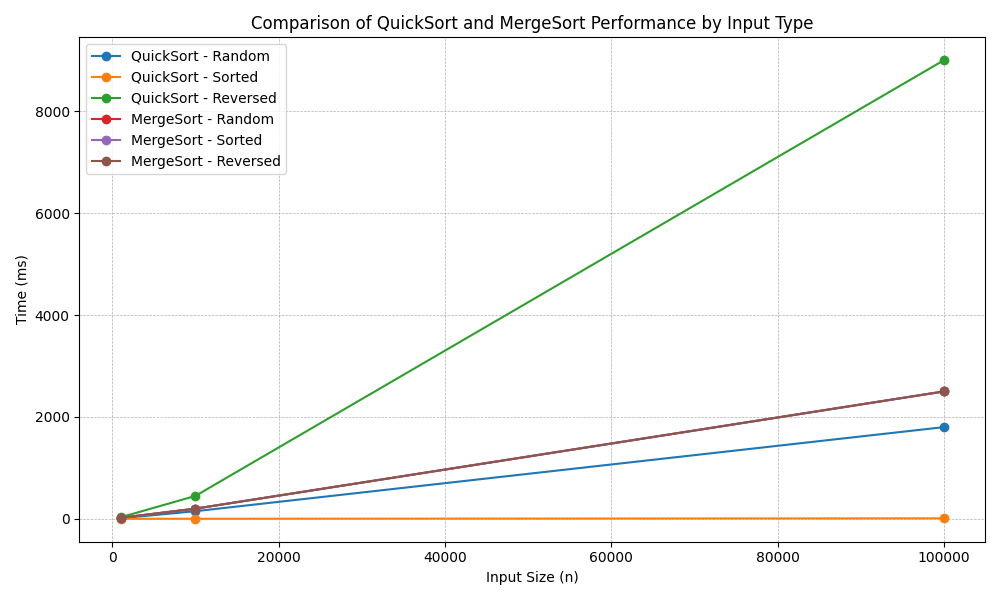
\includegraphics[width=0.8\textwidth]{plot_sort_linear.png}
    \caption{Exekveringstid för de två sorteringsalgoritmerna QuickSort och MergeSort i Scala. För båda algoritmerna plottas tre olika indatatyper separat: Slumpmässig, sorterat och omvänt sorterad indata. \textbf{(Linjär skala)}}
    \label{fig:plot_sort_linear}
\end{figure}
\begin{figure}
    \centering
    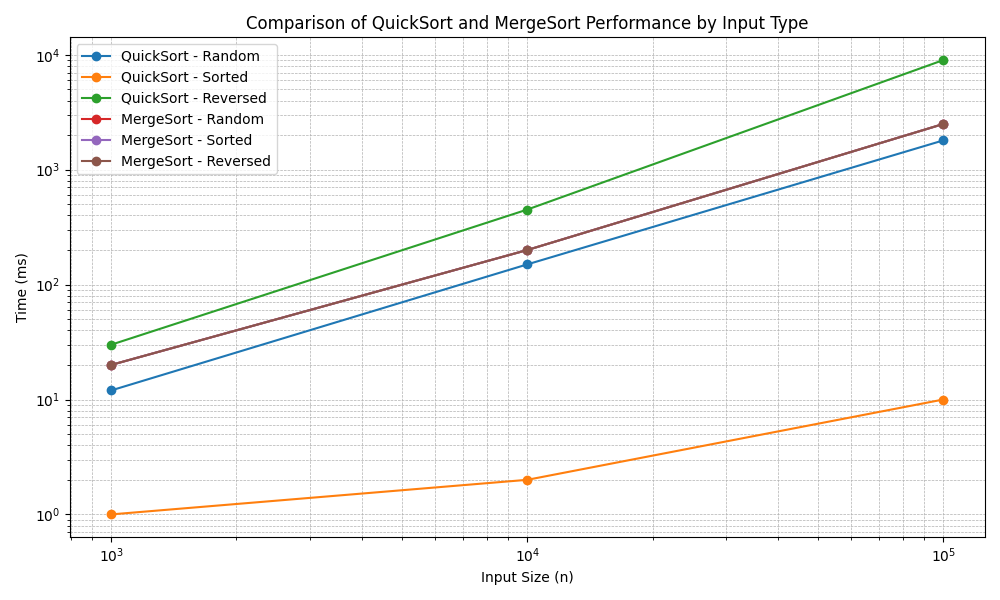
\includegraphics[width=0.8\textwidth]{plot_sort_log.png}
    \caption{Exekveringstid för de två sorteringsalgoritmerna QuickSort och MergeSort i Scala. För båda algoritmerna plottas tre olika indatatyper separat: Slumpmässig, sorterat och omvänt sorterad indata. \textbf{(Logaritmisk skala)}}
    \label{fig:plot_sort_log}
\end{figure}

\newpage

\section{Matematisk analys av algoritmer}

Den matematiska analysen av dessa algoritmer kan göras med hjälp av deras tidskomplexitet. För QuickSort är den förväntade tidskomplexiteten:

\[
    T_Q(n) = O(n \log n)
\]

Medan för MergeSort har vi:

\[
    T_M(n) = O(n \log n)
\]

De har alltså samma tidskomplexitet i det genomsnittliga fallet.
Trots liknande teoretisk prestanda kan dock det praktiska utförandet variera beroende på storlek och typ av indata, som vi såg i tabell~\ref{tab:sorteringsalgoritmer} och figurerna~\ref{fig:plot_sort_linear} och~\ref{fig:plot_sort_log}.

\section{Slutsats}

Vi har undersökt två olika sorteringsalgoritmer i Scala och jämfört deras prestanda. Resultaten visar att valet av algoritm kan ha en betydande påverkan på programmets effektivitet. Genom att förstå dessa skillnader kan utvecklare fatta mer informerade beslut när de designar och optimerar sina program.

\newpage

\appendix
\section{Implementation i Scala}
\label{app:scala_impl}

I kodlistning \ref{lst:scala_example} nedan är ett exempel på en implementation av QuickSort och MergeSort i Scala:

\lstinputlisting[language=Scala,label=lst:scala_example,caption={Scala-program med implementation av QuickSort och MergeSort.}]{sort.scala}


\end{document}
